\cotefile{12}
\scanpage{22}
% archive sheet number: 21
% Several mathematical slots in this typescript were never filled: spacing below preserves them without supplying symbols.
% A long oblique cancellation crosses the Remplaçant paragraph; its exact upper scope is uncertain.
% The pale upper extension is visible between the second and third lines. No verbal text is supplied in the empty formula slots.
\rlap{O}now by reason of flatness $H'_i=\underline{\mathrm{Hom}}\,(\underline{O}_{X'}/J',G'_i)$, hence one can conside\unsure{r} (at the cost of replacing the $G_i$ by the $H_i$) that the $G_i$ are annihilated by $J$. \deleted{Replacing $X$ now by $\operatorname{Spec}(\underline{O}_X/\underline{J})$, one is reduced to the case where $F$ is a faithful Module, hence $X$ is irreducible with generic point the unique point $x\quad\operatorname{Ass}F$. By virtue of the generic flatness theorem, there exists an open \rlap{U}affine neighbourhood $U$ of $x$ such that the ring of its inverse image $U'$ in $X'$ is \uline{free} over that of $U$. Passing \deleted{\unsure{to the|in}} to the interpretation in terms of modules over these rings, one then sees at once that \deleted{on $U'$, the intersection of the} $\quad{}'$ is zero on $U'$. Now by virtue of \unsure{\rlap{\S}paragraph|paragraph} \handwritten{3.3.} one has $\operatorname{Ass}F'\quad X'_x\quad U'$, hence $\quad{}'=0$, Suppose now $n\quad 1$, \mbox{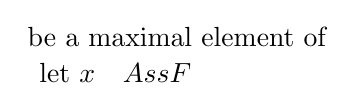
\begin{tikzpicture}[baseline=(base.base),x=1cm,y=1cm]
\node[anchor=west,inner sep=0] (base) at (0,0) {let $x\quad\operatorname{Ass}F$};
\node[anchor=west,inner sep=0] at (-.15,.45) {\inserted{be a maximal element of}};
\end{tikzpicture}}, by what precedes, \deleted{there exists a neighbourhoo} if $U$ is an open neighborhood of $x$ containing no other \unsure{\rlap{l}element|Element|element} of $\operatorname{Ass}F$, $U'$ its inverse image in $U$, then one has $\quad{}'\ U'=0$. In other words, if $i\colon U\quad X$ is the canonical immersion, and $v\colon F\quad i\ (F\ U)$ the canonical homomorphism, hence the transform under $\otimes_X X'$ is identified with $v'\colon F'\quad \rlap{\(v\)}i'\ (F'\ U')$, \deleted{then} (reference), then $\quad{}'$ is a section of $\operatorname{Ker}v'=\operatorname{Ker}v\otimes_X X'$ (flatness again). Introducing $F_1=\operatorname{Ker}v$, one can therefore regard $\quad{}'$ as a section of $F'_1$, and one is reduced to the preceding problem with $F$ replaced by $F_1$. But $\operatorname{Ass}F_1=\operatorname{Ass}F-x$, and one wins by the induction hypothesis. (NB instead of inducting on $\operatorname{card}\operatorname{Ass}$ one can also in this last argument envisage that one has carried out a \deleted{on} noetherian induction on $\operatorname{supp}F$, which is rather more natural and dispenses with checking a silly formula on $\operatorname{Ass}F_1$).}

Of course, proposition \handwritten{3} a) (ii) follows from this, for there one may suppose $X$ and $X'$ affine, the $Z_i$ affine (at the cost of replacing each $Z_i$ by affine opens covering it), and one applies criterion 1. (iii) noting that the $u_i\ (\underline{O}_{Z_i})$ are indeed quasi-coherent.
